\documentclass[12pt]{article}
\usepackage[utf8]{inputenc}
\usepackage{amsmath,amssymb}
\usepackage{amsthm}
\usepackage[nice]{nicefrac}
\usepackage{booktabs}
\usepackage{graphicx}
\usepackage{caption}
\usepackage{lmodern,textcomp}
\usepackage{float}
\usepackage{url}
\usepackage{tabularx}
\renewcommand{\tabularxcolumn}[1]{>{\small}m{#1}}
\usepackage{romannum}
\bibliographystyle{plain}
\usepackage{parskip}
\usepackage{hyperref}

\setlength{\parindent}{0em}
\linespread{1.25}
\newcommand\diff{\,\mathrm{d}}
\renewcommand{\thesubsection}{\arabic{subsection}.}
\renewcommand{\thesubsubsection}{\roman{subsubsection}.}

\usepackage[margin=1.1in]{geometry}
\usepackage{siunitx}
\usepackage[numbers,sort&compress]{natbib}
\usepackage{xcolor}
\usepackage{listings}
\lstdefinestyle{lfonts}{
  basicstyle   = \footnotesize\ttfamily,
  stringstyle  = \color{purple},
  keywordstyle = \color{blue!60!black}\bfseries,
  commentstyle = \color{olive}\scshape,
}
\lstdefinestyle{lnumbers}{
  numbers     = left,
  numberstyle = \tiny,
  numbersep   = 1em,
  firstnumber = 1,
  stepnumber  = 1,
}
\lstdefinestyle{llayout}{
  breaklines       = true,
  tabsize          = 2,
  columns          = flexible,
}
\lstdefinestyle{lgeometry}{
  xleftmargin      = 20pt,
  xrightmargin     = 0pt,
  frame            = tb,
  framesep         = \fboxsep,
  framexleftmargin = 20pt,
}
\lstdefinestyle{lgeneral}{
  style = lfonts,
  style = lnumbers,
  style = llayout,
  style = lgeometry,
}
\lstdefinestyle{python}{
    language = {Python},
    style    = lgeneral,
}

\begin{document}
\pagenumbering{arabic}
\title{How does obesity cases densities affect allocation of funding to London local authorities in 2018}
\author{CASA 0005 Quantitative Methods Coursework 1}
\date{November 15, 2020}
\maketitle
\subsection{Introduction}
NHS claimed almost one in five Year 6 children in the UK was found to be obese in 2018, and sadly this number is not dropping during the past few years. The origins of childhood obesity stem from various aspects, including lifestyle, genetic and environmental issues. The government has been taking considerable forms of actions to tackle this problem, from sugar reduction to advertising and promotions. This study investigates how government has been allocating their funding, in particular, to local authorities in London.


\subsection{Data}
The data used in this study contains population, obesity cases, total budget, and allocation of funding for local authorities across London in 2018. An illustration of data employed is shown in Table \eqref{t1}. 
\begin{table}[H]

\begin{center}
\resizebox{\textwidth}{!}{%
\begin{tabular}{c|c|c|c|c|c|c|c}
% {|*{15}{>{\centering\arraybackslash}X|}}
\hline

 & local authorities & total obesities & total population & obesity density & ... & total budget & ... \\ \hline
0 & Barking and Dagenham & $763$ & $181779$ & $0.420$ & ... & $139000$ & ... \\ \hline
1 & Barnet & $773$ & $355955$ & $0.217$ & ... & 220000 & ... \\ \hline
 \multicolumn{7}{c}{\vdots} \\ \hline
\end{tabular}}
\captionsetup{font=scriptsize}
\caption{Illustration of data used, list of column names{} include: \newline
Names of local authority areas; total obesity cases in each area; total population; obesity density per 100 people (obesity cases divided by population multiplied by 100); total budget allocated (in pounds); percent of budget spent on improving air quality, cleaner environment, health training, raising school awareness, media awareness and subsiding counselling.
} \label{t1}
\end{center}
\end{table}

Only one observation is considered an outlier due to its relatively small scale, City of London data,  therefore is dropped from the dataset. Its population is below the average population in London boroughs by $97\%$, having this data in the linear regression plot of obesity density vs. total budget lowers the regression coefficient from $0.437$ to $0.349$. 


\subsection{Methodlogy}
Three approaches were taken to investigate the criteria of funding:

\romannum{1}. 
A linear line was fitted using scipy.stats.linregress() between obesity density and total budget spent. 


\romannum{2}.
A more outlier-robust linear approach, called Random Sample Consensus (RANSAC) was used. This method compliments the ordinary least squares methods by adding detections of outliers and accord them to have no influence on the parameters of the model (Fischler and Bolles, 1981). In \verb|sklearn.linear_model.RANSACRegressor()|, outliers are classified as those whose residual exceed the median absolute deviation of dependent variables (Pedregosa, F. et al., 2011).

\romannum{3}.
Finally, a non-linear approach was taken. Polynomial regression of various degrees was fitted to the data using \verb|numpy.polyfit()| in Python. 


\subsection{Results}
\romannum{1}. Logically one might assume that the more obesity cases discovered per unit population, the more funding should be allocated. 
The linear line fitted to obesity density vs. total budget spent yields a coefficient of determination of $0.002$, which means that only $0.2\%$ of the variance of dependent variable (total budget) is explained by independent variable (obesity density). Log transformations were also applied to the variables, associated parameters are shown in Table \eqref{t2}. 


\begin{table}[H]
\begin{center}
\resizebox{\textwidth}{!}{%
\begin{tabular}{|l|c|c|c|c|}
\hline
 &	unchanged data &$log(x)$ and y&$log(y)$ and x&	$log(x)$ and $log(y)$	 \\ \hline
slope &	$9.9e7$ & $9.6e5$ & $49$ & $5.07$\\ \hline

constant	& $1.6e5$ & $-3.1e5$ & $12$ & $9.47$ \\ \hline

$R^2$	&$0.037$ &$0.29$ & $0.032$ & $0.29$\\ \hline

Pearson correlation coefficient & $0.19$ & $0.537$ &$0.18$ & $0.536$  \\ \hline

p value & $0.29$ & $0.001$ & $0.32$ & $0.002$ \\ \hline

relationship implied & linear   & exponential & exponential  & power \\ \hline
\end{tabular}}
\captionsetup{font=scriptsize}
\caption{coefficients related to the relationship between original and log-transformed obesity density (x) and total budget spent(y)} \label{t2}
\end{center}
\end{table}

As the maximum value of $R^2$ being under $0.3$ in Table \eqref{t2}, the amount of funding allocated is extremely weakly correlated with the obesity cases per unit population by the power law. No relationship is within the accepted range of $R^2 \geq 0.5$ or $p \leq 0.05 $, thus indicating there is no meaningful linear, exponential, or power law relationships between them. 


\romannum{2}.
The lack of a meaningful linear relationship could be induced by number of outliers involved. The outliers in this case originate from changes in human behaviour, the government may identify some boroughs need more attention due to reasons that cannot be shown in statistical measures. Building from the results in \romannum{1}, log transformed data has been used to plot Figure \eqref{RANSAC}, where in \verb|RANSAC|, a considerable proportion of data has been classified as outliers due to its randomness and large variance of human behaviours. 

% \begin{figure}[H]
% \begin{center}
% 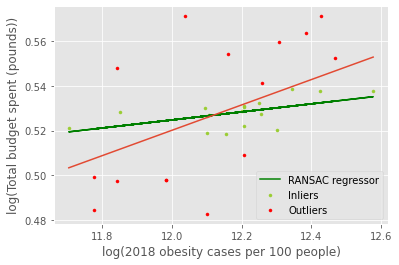
\includegraphics[scale=0.45]{RANSAC.png}
% \captionsetup{font=scriptsize}
% \caption{$log($total budget$)$ vs. $log($obesity density$)$ plot, linear relationship obtained from Ordinary Least Squares(red) and RANSAC(green). RANSAC is only fitting to inliers, while OLS is fitting to all data.}\label{RANSAC}
% \end{center}
% \end{figure}

\begin{figure}[!htb]
   \begin{minipage}{0.48\textwidth}
     \centering
     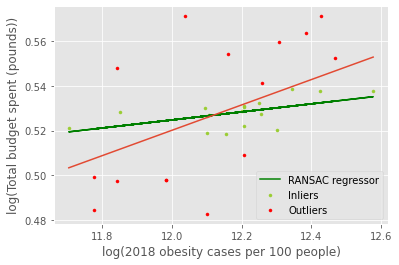
\includegraphics[width=.95\linewidth]{RANSAC.png}
     \captionsetup{font=scriptsize}
     \caption{$log($obesity density$)$ vs. $log($total budget$)$ plot, linear relationship obtained from Ordinary Least Squares(red) and RANSAC(green). RANSAC is only fitting to inliers, while OLS is fitting to all data.}\label{RANSAC}
   \end{minipage}\hfill
   \begin{minipage}{0.48\textwidth}
     \centering
     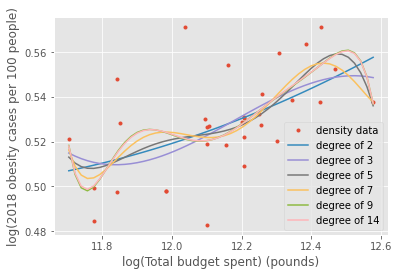
\includegraphics[width=.95\linewidth]{poly.png}
     \captionsetup{font=scriptsize}
     \caption{Fitting various degrees of polynomials to $log($obesity density$)$ vs. $log($total budget$)$ plot. All logs in this paper refer to the natural log.}\label{Poly}
   \end{minipage}
\end{figure}

Although RANSAC increased $R^2$ from $0.29$ to $0.39$, p value has surmounted past the acceptable range. Visually, the rise of $R^2$ is explained by the excessive amount of outliers removed. Additionally, the classification of outliers is entirely statistical and without contextual reasons, it is difficult to examine whether the outliers could otherwise play an essential part on the overall trend. To summarise, the criteria of identifying outliers in RANSAC approach is stricter and less stable, thus making it a less reliable method. 


\romannum{3}. 
Selected degrees of 2 to 6 of polynomial regression are shown in Figure  \eqref{Poly}, and associated $R^2$ values are displayed in Table \eqref{t3}. 

% \begin{figure}[H]
% \begin{center}
% 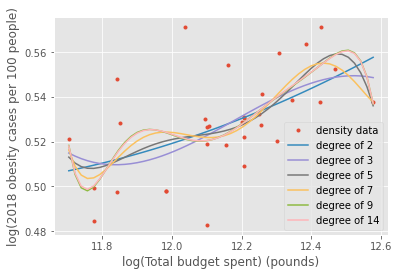
\includegraphics[scale=0.45]{poly.png}
% \captionsetup{font=scriptsize}
% \caption{Fitting various degrees of polynomials to $log($total budget$)$ vs. $log($obesity density$)$ plot. Both logs refer to the natural log.}\label{Poly}
% \end{center}
% \end{figure}

\begin{table}[H]
\begin{center}
\resizebox{\textwidth}{!}{%
\begin{tabular}{|l|c|c|c|c|c|c|}
\hline
degrees of polynomial fitted & 1 & 2 & 3 & 4 & 5 & 6   \\ \hline
Coefficient of determination $R^2$ & $0.387$ & $0.307$ & $0.335$ & $0.34$ & $0.342$ & $0.346$ \\ \hline
\end{tabular}}
\captionsetup{font=scriptsize}
\caption{coefficients related to the relationship between original and log-transformed total budget spent and obesity density} \label{t3}
\end{center}
\end{table}

It can be spotted that as the degree of polynomial fitted increases, $R^2$ increases. One could deliberately dial the degree up and manipulate r squared to the range accepted, but this would be an invalid approach logically. By doing so, the model yielded would be highly influenced by the noise in the dataset, rather than demonstrating its underlying real trend. Furthermore, $R^2$ starts to converge when hitting degree of 7, and a warning message is generated when fitting above this, suggesting that \verb|Polyfit()| may be poorly conditioned. The $R^2$ value that optimises the bias-variance trade-off is near $0.35$, this is still not enough to indicate an appropriate polynomial relationship. 

\subsection{Conclusion}

To conclude, there is no strong statistical relationship between obesity density and total budget. Neither a simple OLS nor an outlier-robust yet unstable RANSAC linear approach has correctly identify any relationships. There is no appropriate polynomial relationship that could balance bias-variance trade-off either. Another approach to examine the criteria of allocating funding is to consider the relationship of total budget with population and number of obesity cases respectively. Interestingly, there is a strong power law relationship when fitting between the above variables. Additionally, no multiple linear relationship is found between areas of spending the budget and obesity density by plotting the correlation matrix. The above results have been omitted from this study for brevity. Further research could be conducted to investigate the reasons of such behaviours. 

Another question could be raised is whether the obesity problem is alleviated with more budget spent by exchanging the dependent and independent variables. Bearing in mind that a reference level of obesity density expansion, which arises from an existing annual increase of obesity density along with population increase, should be obtained beforehand. This reference level could be calculated from different budget spent in previous years and associated obesity densities. 

\subsection{Appendix}
Python code used to generate the figures and calculate the relevant data, as well as \LaTeX\  source code used to generate this report can be found at: \url{https://github.com/Tiana125/CASA0005_QM_CW1}


\newpage

\appendix

\bibliography{CW1}

Fischler, M. A. and Bolles, R. C. (1981). ‘Random sample consensus: a paradigm for model fitting with applications to image analysis and automated cartography’. Communications of the ACM, 24 (6), pp. 381–395. doi: 10.1145/358669.358692.


NHS. (2018). National Child Measurement Programme, England 2018/19 School Year. Available at: https://digital.nhs.uk/data-and-information/publications/statistical/national-child-measurement-programme/2018-19-school-year.


Pedregosa, F., Varoquaux, G., Gramfort, A. and Michel, V. (2011). ‘Scikit-learn: Machine Learning in Python’. Journal of Machine Learning Research, (12), pp. 2825–2830.


\end{document}